\chapter{Comunicando Arduino con otros sistemas}

Hoy en día la manera más común de comunicación entre dispositivos electrónicos es la comunicación serial y Arduino no es la excepción. A través de este tipo de comunicación podremos enviar datos a y desde nuestro Arduino a otros microcontroladores o a un computador corriendo alguna plataforma de medios (Processing, PD, Flash, Director, VVVV, etc.). En otras palabras conectar el comportamiento del sonido o el video o un programa monitor a sensores o actuadores. Explicaré aquí brevemente los elementos básicos de esta técnica:
\section{Funciones básicas}
El mismo cable con el que programamos el Arduino desde un computador es un cable de comunicación serial. Para que su función se extienda a la comunicación durante el tiempo de ejecución, lo primero es abrir ese puerto serial en el programa que descargamos a Arduino. Para ello utilizamos la función:
\begin{lstlisting}
Serial.begin(9600);
\end{lstlisting}
Ya que solo necesitamos correr esta orden una vez, normalmente iría en el bloque void setup(). El número que va entre paréntesis es la velocidad de transmisión y en comunicación serial este valor es muy importante ya que todos los dispositivos que van a comunicarse deben tener la misma velocidad para poder entenderse. 9600 es un valor estándar y es el que tienen por defecto Arduino al iniciar.\\º
Una vez abierto el puerto lo más seguro es que luego queramos enviar al computador los datos que vamos a estar leyendo de uno o varios sensores. La función que envía un dato es:
\begin{lstlisting}
Serial.print(data);
\end{lstlisting}
Una mirada en la referencia de Arduino permitirá constatar que las funciones print y println (lo mismo que la anterior pero con salto de renglón) tienen opcionalmente un modificador que puede ser de varios tipos:
\begin{itemize}
\item Serial.print(data, DEC);   // decimal en ASCII
\item Serial.print(data, HEX);   // hexadecimal en ASCII 
\item Serial.print(data, OCT);    // octal en ASCII 
\item Serial.print(data, BIN);    // binario en ASCII 
\item Serial.print(data, BYTE);   // un Byte
\end{itemize}
Como puede verse, prácticamente todos los modificadores, menos uno, envían mensajes en ASCII. Explicaré brevemente:
\section{Series de pulsos}
En el modo más sencillo y común de comunicación serial (asincrónica, 8 bits, más un bit de parada) siempre se está enviando un byte, es decir un tren de 8 pulsos de voltaje legible por la máquina como una serie de 8 bit (1 ó 0):

\begin{figure}[!htp]
	\centering
	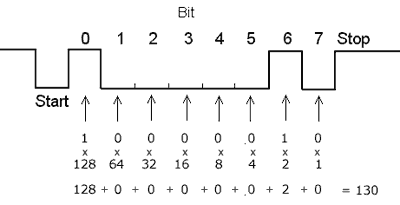
\includegraphics[width=200pt]{./Imagenes/Documentos/ArduinoNotebook_img12.png}
	\caption[Series de pulsos]{Series de Pulsos}
\end{figure}
O sea que no importa cual modificador usemos siempre se están enviando bytes. La diferencia esta en lo que esos bytes van a representar y sólo hay dos opciones en el caso del Arduino: una serie de caracteres ASCII o un número.\\
Si Arduino lee en un sensor analógico un valor de 65, equivalente a la serie binaria 01000001 esta será enviada, según el modificador, como:
\begin{table}[!htp]
	\begin{tabular}{|l|l|l|}
		\hline
		dato & Modificador    &     Envío (pulsos) \\
		\hline
		65  &  DEC  & ('6' y '5'' ASCIIs 54–55)\\
		\hline
		65  &  HEX  & ('4' Y '1' ASCIIs 52–49)\\
		\hline  
		65  &  OCT  & ('1', '0' y '1' ASCIIs 49–48–49)\\
		\hline 
		65  &  BIN  & ('0','1','0','0','0','0','0'y '1'   ASCIIs 49–48–49–49–49–49–49–48)\\
		\hline
		65  &  BYTE & 01000001 \\
		\hline
     \end{tabular}
	 \caption{Equivalencia a binario}
\end{table}
No explicaremos conversiones entre los diferentes sistemas de representación numérica, ni la tabla ASCII, pero es evidente como el modificador BYTE permite el envío de información más económica (menos pulsos para la misma cantidad de información) lo que implica mayor velocidad en la comunicación. Y ya que esto es importante cuando se piensa en interacción en tiempo real es el modo que usaremos.
\section{Un ejemplo sencillo}
Enviar un sólo dato es realmente fácil. En el típico caso de un potenciómetro conectado al pin 2 de Arduino:
\begin{lstlisting}
int potPin = 2;
int ledPin = 13;
int val = 0;

void setup()
{
   Serial.begin(9600);
   pinMode(ledPin, OUTPUT);
   digitalWrite(ledPin, HIGH); //activamos el pin para saber cuando arranco
}

void loop()
{
   val = analogRead(potPin);     // lee el valor del Pot
   Serial.println(val);
}
\end{lstlisting}
Si no utilizamos ningún modificador para el Serial.println es lo mismo que si utilizáramos el modificador DEC. Así que no estamos utilizando el modo más eficiente pero si el más fácil de leer en el mismo Arduino. Al ejecutar este programa podremos inmediatamente abrir el monitor serial del software Arduino (último botón a la derecha) y aparecerá el dato leído en el potenciómetro tal como si usáramos el println en Processing.
Envío a Processing (versión ultra simple)
Para enviar este mismo dato a Processing si nos interesa utilizar el modo BYTE así que el programa en Arduino quedaría así:
\begin{lstlisting}
int potPin = 2;
int ledPin = 13;
int val = 0;

void setup()
{
   Serial.begin(9600);
   pinMode(ledPin, OUTPUT);
   digitalWrite(ledPin, HIGH); // activamos el pin para saber cuando arranco
}

void loop()
{
   // lee el Pot y lo divide entre 4 para quedar entre 0-255
   val = analogRead(potPin)/4;
   Serial.print(val, BYTE);
}
\end{lstlisting}
En Processing tenemos que crear un código que lea este dato y haga algo con él:
\begin{lstlisting}
import processing.serial.*;

Serial puerto; // Variable para el puerto serial
byte pot; // valor entrante
int PosX;

void setup()
{
   size(400, 256);
   println(Serial.list()); // lista los puertos seriales disponibles

   //abre el primero de esa lista con velocidad 9600
   port = new Serial(this, Serial.list()[0], 9600);
   fill(255,255,0);
   PosX = 0;
   pot = 0;
}

void draw()
{
   if(puerto.available() > 0) 
   { // si hay algun dato disponible en el puerto
     pot = puerto.read(); // lo obtiene
     println(pot);
   }
   ellipse(PosX, pot, 3, 3); // y lo usa 
   if (PosX < width)
   {
      PosX++;
   } else { fill(int(random(255)),int(random(255)),int(random(255)));
    PosX = 0;
   }
}
\end{lstlisting}
Si ya se animó a intentar usar más de un sensor notará que no es tan fácil como duplicar algunas líneas.
\section{Comunicación vía puerto Serie:}

La tarjeta Arduino puede establecer comunicación serie (recibir y enviar valores codificados en ASCII) con un dispositivo externo, a través de una conexión por un cable/puerto USB o cable/puerto serie RS-232.\\
Igual que para la descarga de los programas, sólo será necesario indicar el número de puerto de comunicaciones que estamos utilizando y la velocidad de transferencia en baudios.También hay que tener en cuenta las limitaciones de la transmisión en la comunicación serie, que sólo se realiza a través de valores con una longitud de 8-bits (1 Byte)(ver Serial.write() o Serial.read(c) ), mientras que como ya se hemos indicado, el A/D (Convertidor) de Arduino tiene una resolución de 10-bits.(enlace)\\
Dentro del interfaz Arduino, disponemos de la opción 'Monitorización de Puerto Serie', que posibilita la visualización de datos procedentes de la tarjeta.
\begin{figure}[!htp]
	\centering
	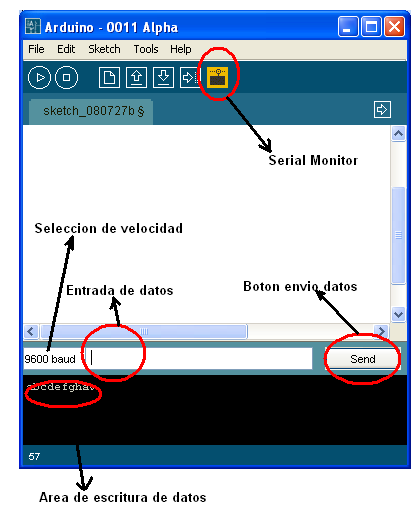
\includegraphics[width=200pt]{./Imagenes/Documentos/ArduinoNotebook_img13.png}
	\caption[Series de pulsos]{Series de Pulsos}
\end{figure}
Para definir la velocidad de transferencia de datos, hay que ir al menú 'Herramientas' (Tools) y seleccionar la etiqueta 'Velocidad de monitor Serie'(Tools). La velocidad seleccionada, debe coincidir con el valor que hemos determinado o definido en nuestro programa y a través del comando Serial.begin().Dicha velocidad es independiente de la velocidad definida para la descarga de los programas.\\
La opción de 'Monitorización de puerto serie' dentro del entorno Arduino, sólo admite datos procedentes de la tarjeta. Si queremos enviar datos a la tarjeta, tendremos que utilizar otros programas de monitorización de datos de puerto serie como HyperTerminal (para Windows) -Enlace o ZTerm (para Mac)-XXXX- Linux-Enlace, etc.\\
También se pueden utilizar otros programas para enviar y recibir valores ASCII o establecer una comunicación con Arduino: Processing (enlace), Pure Data (enlace), Director(enlace), la combinación o paquete serial proxy + Flash (enlace), MaxMSP (enlace), etc.\\
Nota: Hay que dejar tiempos de espera entre los envíos de datos para ambos sentidos, ya que se puede saturar o colapsar la transmisión.\\
\newpage{}
\section{Envío de datos desde Arduino(Arduino->PC) al PC por puerto de comunicación serie:}

Ejercicio de volcado de medidas o valores obtenidos de un sensor analógico\\
\textbf{Código}
\begin{lstlisting}
/* Lectura de una entrada analogica en el PC
El programa lee una entrada analogica, la divide por 4
para convertirla en un rango entre 0 y 255, y envia el valor al PC en diferentes formatos ASCCI.
A0/PC5: potenciometro conectado al pin analogico 1 y puerto de PC-5
Created by Tom Igoe 6 Oct. 2005
Updated
*/

int val; // variable para capturar el valor del sensor analogico

void setup()
{
   // define la velocidad de transferencia a 9600 bps (baudios)
   beginSerial(9600);
}

void loop()
{
   // captura la entrada analogica, la divide por 4 para hacer el rango de 0-255
   val = analogRead(0)/4;

   // texto de cabecera para separar cada lectura:
   printString('Valor Analogico =');

   // obtenemos un valor codificado en ASCII (1 Byte) en formato decimal :
   printInteger(val);
   printString('\t'); //Caracter espacio

   // obtenemos un valor codificado en ASCII (1 Byte) en formato hexadecimal :
   printHex(val);
   printString('\t');

   // obtenemos un valor codificado en ASCII (1 Byte) en formato binario
   printBinary(val);
   printString('\t');

   // obtenemos un valor codificado en ASCII (1 Byte)en formato octal:
   printOctal(val);
   printString('\n\r'); //caracter salto de linea y retorno de carro

   // espera 10ms para la proxima lectura
   delay(10);
}
\end{lstlisting}
Otra solución puede ser la de transformar los valores capturados en un rango entre 0 y 9 y en modo de codificación ASCII o en caracteres ASCII. De forma que dispongamos de un formato más sencillo o legible, sobre la información capturada.\\
El siguiente código incluye una función llamada \textbf{treatValue()} que realiza dicha transformación.
\begin{lstlisting}
int val; // variable para capturar el valor del sensor analogico

void setup()
{
   // define la velocidad de transferencia a 9600 bps (baudios)
   beginSerial(9600);
}

int treatValue(int data)
{
   return (data * 9 / 1024) + 48; //formula de transformacion
}

void loop()
{
   val= analogRead(0); //captura del valor de sensor analogico (0-1023)
   serialWrite(treatValue(val)); //volcado al puerto serie de 8-bits
   serialWrite(10); //caracter de retorno de carro
   serialWrite(13); //caracter de salto de linea
   delay(10); 
}

// Serial Output 
// by BARRAGAN <http://people.interaction-ivrea.it/h.barragan>

int switchpin = 0; // interruptor conectado al pin 0

void setup()
{
   pinMode(switchpin, INPUT); // pin 0 como ENTRADA
   Serial.begin(9600);    // inicia el puerto serie a 600bps
}

void loop()
{
   if(digitalRead(switchpin) == HIGH) //si el interruptor esta en ON
   {
      Serial.print(1);    // envia 1 a Processing
   } else {
      Serial.print(0);    // en caso contrario envia 0 a Processing
   }
   delay(100);     // espera 100ms
}
\end{lstlisting}